\chapter{ Autoencoder }
% Authors: Bixing Yan (by783), Chengze Zuo (cz1565) , Yavuz Sunor (ys3226) Apr 14, 2019.
\section{ Introduction }
\\
Autoencoders are one of two(the other is Generative Adversarial Networks) most commonly used and efficient Generative models approaches. Generative models are unsupervised(semi) learning algorithms aiming at learning the true data distributions of the training set so as to generate new data points with some variations. They are widely used in image processing to create super resolutions when zooming into low pixel images and also in inpainting and image captioning.
\\
Autoencoder is a an unsupervised learning of efficient data coding. With neural network layers as encoder and decoder, the aim of an autoencoder is to restore its input data at the output. Traditionally, autoencoders are used for dimensionality reduction; while recently, this concept are more widely used for learning the generative model of data.
\\
The schematic illustration is shown as below:
\\
\begin{figure}[htb]
    \centering
    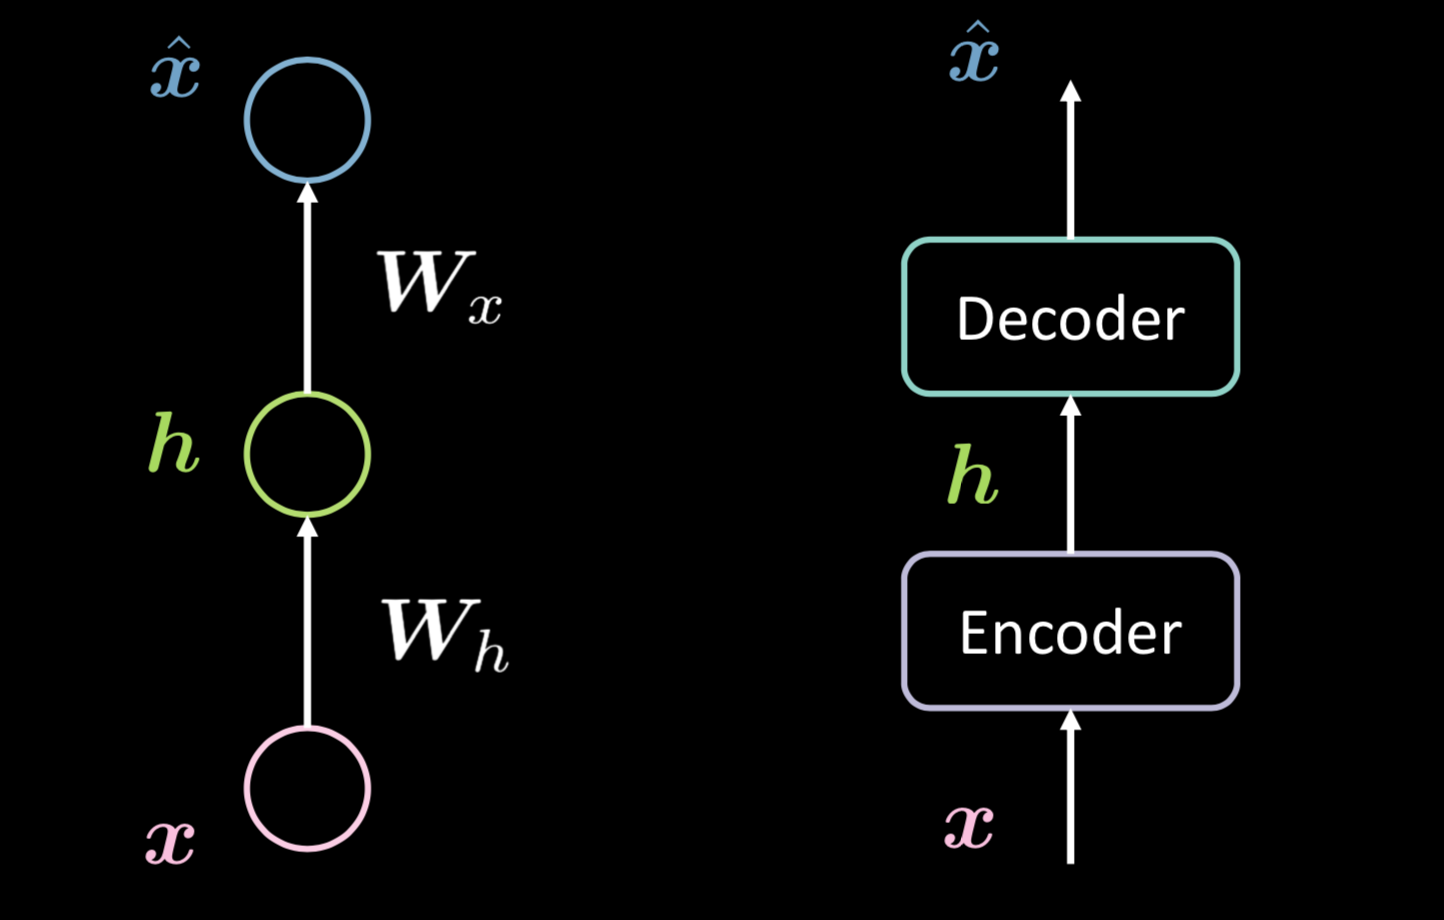
\includegraphics[width=0.6\textwidth]{labs/09/images/Schematic_Illustration_of_Autoencoder.png}
    \caption{Schematic Illustration of Autoencoder}
    \label{fig:Schematic_Illustration_of_Autoencoder}
\end{figure}
\\
From the above figure, we can know, typically, an autoencoder consists two parts: the encoder and the decoder. The encoder will map the input data to a target space (or some would refer as hidden space) ($f_h: x\rightarrow h$), while the decoder will project the data from the target space back to the original input space ($f_x: h\rightarrow \hat{x}$).
\\
The performance of an autoencoder is evaluated by how similar the decoder can restore the data after it is coded by the encoder. Thus, the loss of an autoencoder is inversely correlated with the similarity between the input $x$ and the output $\hat{x}$ (or we might call it as the reconstruction loss). 
$$ L=\frac{1}{m}\sum_{j=1}^m l(x^j,\hat{x}^j) $$
For example, for the binary output, the entropy loss is usually used as the evaluation metric:
$$ l(x,\hat{x}) = -\sum_{i=1}^n[x_i\log(\hat{x}_i) + (1-x_i)\log(1-\hat{x}_i) ]$$
And, for the real value output, the performance of an autoencoder is usually evaluated with the Euclid distance:
$$ l(x,\hat{x}) = \frac{1}{2} \| x-\hat{x} \|^2 $$
By reducing the loss, we can train the autoencoder.
\\
Depending on the dimension of the coded space (hidden layer), the autoencoder can be described as under-complete or over-complete, as the figure shown below:
\\
\begin{figure}[htb]
    \centering
    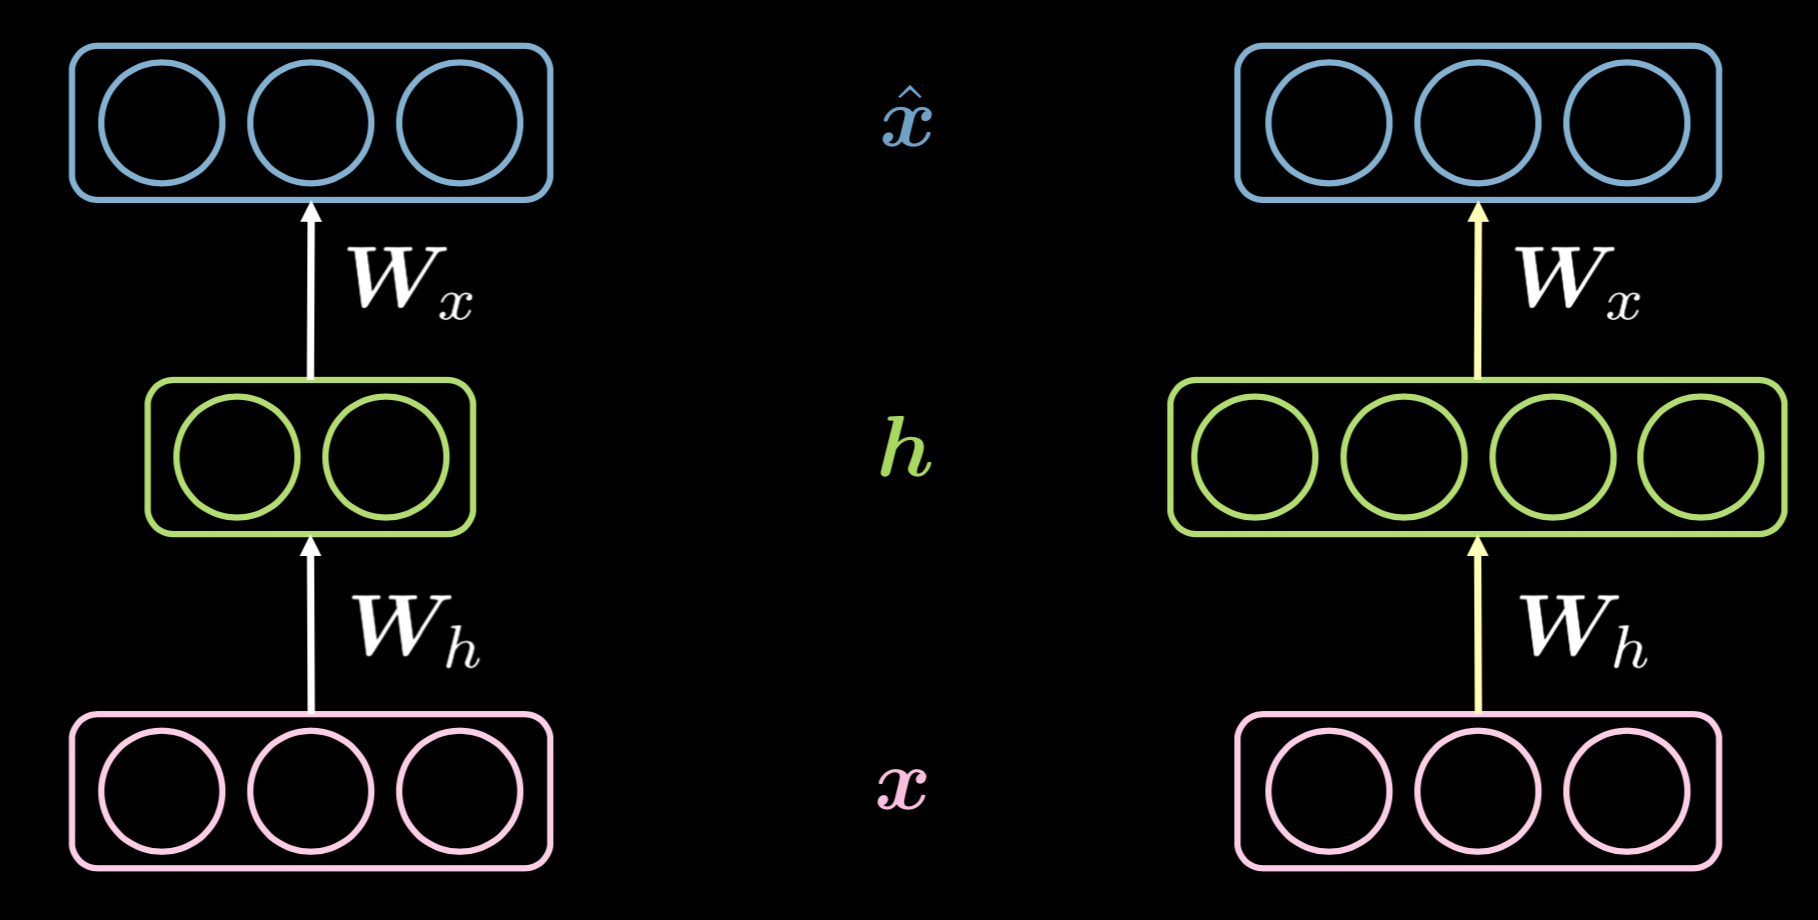
\includegraphics[width=0.6\textwidth]{labs/09/images/Under_(over)_complete_Autoencoder.png}
    \caption{Under-complete (left) and over-complete (right) Autoencoder}
    \label{fig:Under_(over)_complete_Autoencoder}
\end{figure}
\\
As its name, the size of the hidden layer of an under-complete autoencoder will be smaller than the input size; while that of an over-complete one will be large than the input size. The under-complete auto encoder is usually applied to perform dimension reduction, while the over-complete autoencoder is utilized to learn features.

More specific, for an under-complete autoencoder, the dimension of the hidden layer would be smaller than the instrinsic dimension of data manifold (The point here is to learn the feature. If you have same number of neurons, you can just simply copy). So this type of autoencoder will encode features that are important for reconstructing (usually will introduce constraints from previous layers). In other words, by training an under-complete representation, we force the autoencoder to learn the most salient features of the training data. That's why, an under-complete autoencoder will work good when reconstructing samples similar to training samples, but bad with other types of inputs.  

As for over-complete autoencoders, more units in the hidden layer would basically not guarantee that the hidden units will extract meaningful structure,but most likely copy the input element by element. However, if we are interested in a linear classifier, more dimension allows the network to learn more/better features (higher dimension is better). So, for example, this kind of autoencoders wont do well with MNIST dataset which requires non-linearity to learn seperable patterns. Two ways to deal with this problem and extract meaningful features are using denoising and contractive autoencoders.
\\
\subsection{Denoising Autoencoder}
\\
Denoising autoencoders take a partially corrupted input whilst training to recover the original undistorted input. The denoising autoencoder mainly focuses on robust representations of inputs and extracting features that are useful for representation of the input distribution.
\\
As the description above, to train the autoencoder, we need to corrupt the data with small noise ($x \rightarrow x'$). The distribution of the noise will be comparable to our observation in reality, so that the denoising autoencoder can robustly recover the real data.
\\One thing need to note here is, because the ideal output $\bar{x}$ are expected to be the clean data $x$ rather than the noised input $x'$, the loss is a function of $x$ and $\bar{x}$, i.e., $l(x,\bar{x})$ rather than $l(x',\bar{x})$.
\\
A schematic illustration of the corruption and denoising process is shown below:
\\
\begin{figure}[htb]
    \centering
    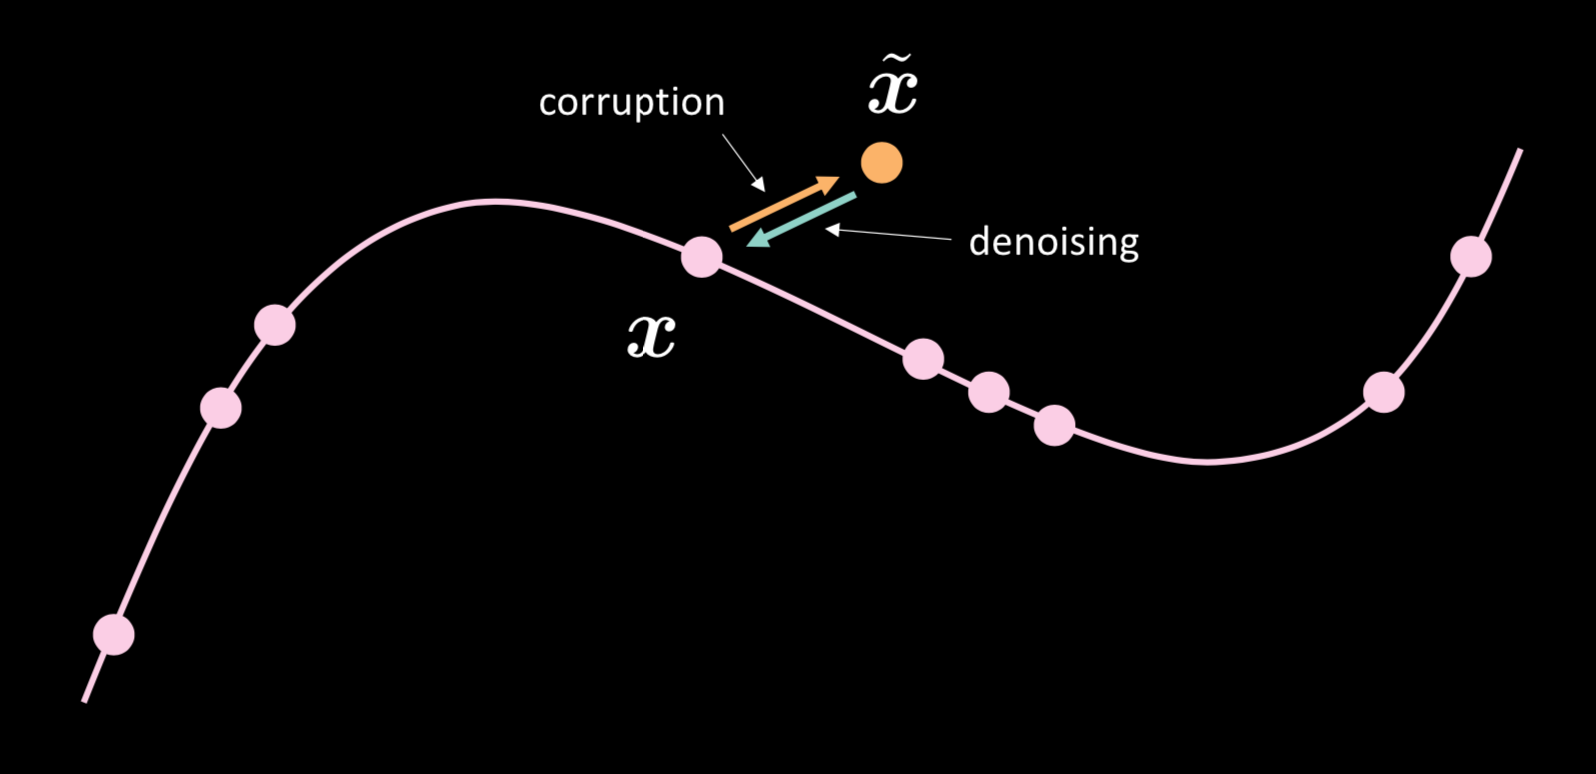
\includegraphics[width=0.6\textwidth]{labs/09/images/Corrpution_and_Denoising.png}
    \caption{Corruption and Denoising Process for Denoising Autoencoder}
    \label{fig:Corrpution_and_Denoising}
\end{figure}

\subsection{Contractive Autoencoder}

A contractive autoencoder makes this encoding less sensitive to small variations in its training dataset. This is achieved by adding an explicit regularizer in the objective function to force the model to learn a function that is robust to slight variations of input values. The loss function includes a term that penalize insensitivity to the reconstruction direction and a term that penalize sensitivity to all directions:

$$l(x,\bar{x}) = l_{\text{reconstruction}} + \lambda \| \nabla_x h \|^2$$
\\
A schematic illustration of this concept is shown below: 
\\
\begin{figure}[H]
    \centering
    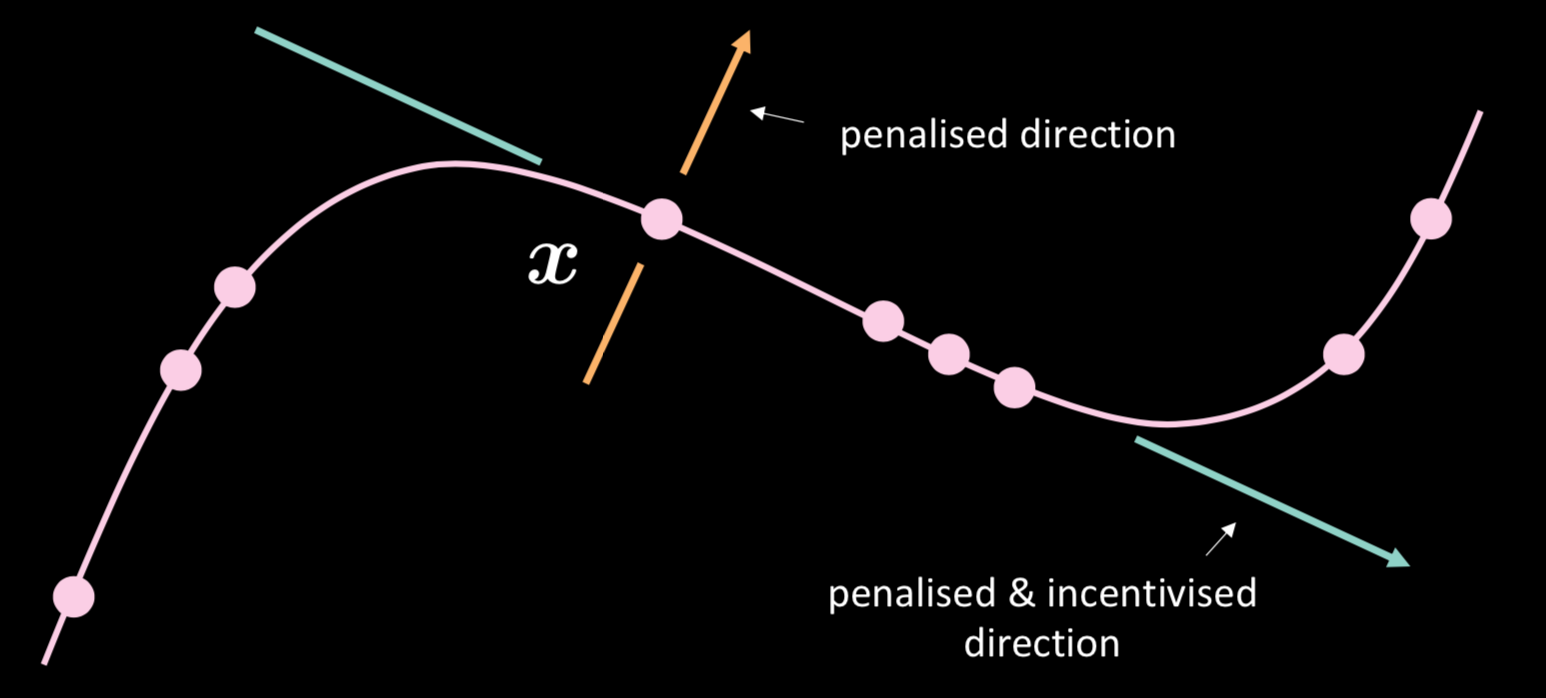
\includegraphics[width=0.6\textwidth]{labs/09/images/Contractive_AutoEncoder.png}
    \caption{Illustration of Penalization on Different Directions}
    \label{fig:Contractive_AutoEncoder}
\end{figure}

\subsection{Data Manifold}

Converting data points from data manifold to latent space \textbf{Z} requires knowing the intrinsic dimension of the input. By unwarping the data from higher dimension into lower dimension, we could have data presented in the hidden/latent layer. If we have start and ending points on the latent space, as well as interpolated point between, we could actually interpolate back into higher dimensional space. But in terms of how we can go back from latent space to the high dimension space, they are quite challenging. Either learning the distribution of data points or enforcing some structure could be a candidate solution.
\\
\begin{figure}[htb]
    \centering
    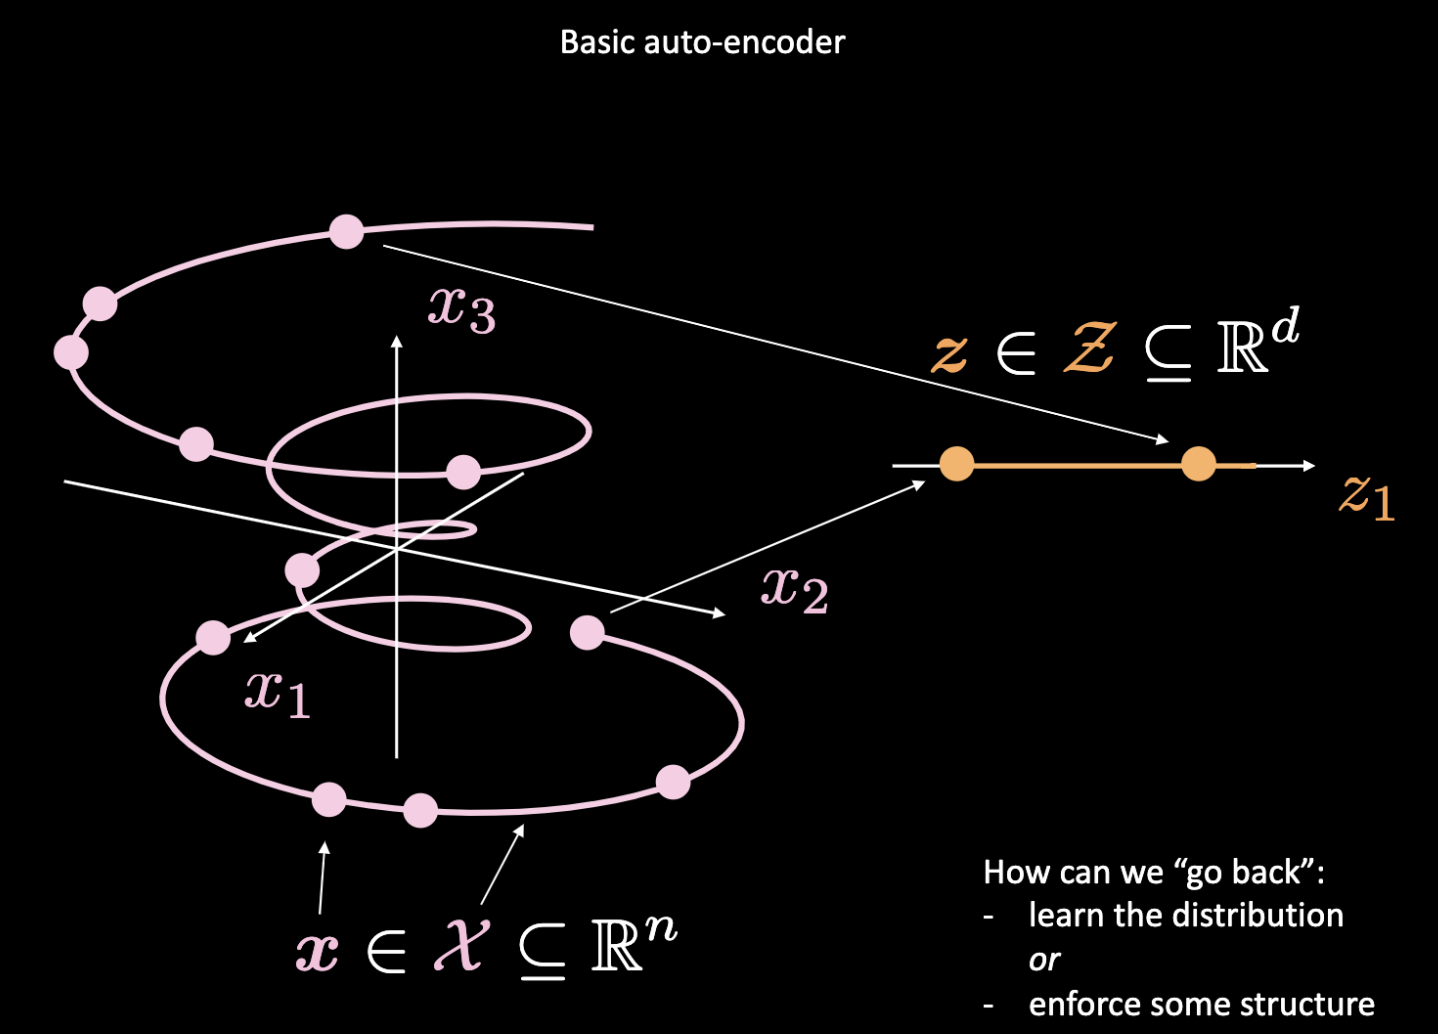
\includegraphics[width=0.6\textwidth]{labs/09/images/Data_manifold.png}
    \caption{Illustration on unwarping data manifold}
    \label{fig:Data_manifold}
\end{figure}
\\





